\documentclass[a4paper,14pt]{extarticle}
\usepackage{../../tex-shared/report-layout}

\renewcommand{\mylabnumber}{6}
\renewcommand{\mylabtitle}{Основы принятия управленческих решений}
\renewcommand{\mysubject}{Управление IT-проектами}
\renewcommand{\mylecturer}{Смирнова Н.Б.}

\begin{document}
\begin{titlepage}
    
    \thispagestyle{empty}
    
    \begin{center}
        
        Министерство науки и Высшего образования Российской Федерации \\
        Севастопольский государственный университет \\
        Кафедра ИС
        
        \vfill

        Отчет \\
        по лабораторной работе №\mylabnumber \\
        \enquote{\mylabtitle} \\
        по дисциплине \\
        \enquote{\MakeTextUppercase{\mysubject}}

    \end{center}

    \vspace{1cm}

    \noindent\hspace{7.5cm} Выполнил студент группы ИС/б-17-2-о \\
    \null\hspace{7.5cm} Горбенко К. Н. \\
    \null\hspace{7.5cm} Проверил \\
    \null\hspace{7.5cm} \mylecturer

    \vfill

    \begin{center}
        Севастополь \\
        \the\year{}
    \end{center}

\end{titlepage}

\section{Цель работы}
Сформировать навыки принятия управленческих решений.

\section{Задание на работу}
Менеджеру проекта по разработке программного продукта необходимо принять решение
о выборе архитектуры разрабатываемого продукта. Имеются две альтернативы:
\begin{enumerate}
    \item можно выбрать простую архитектуру клиент-сервер, причем известно, что
          в этом случае стоимость разработки составит 400 тыс. руб.;
    \item можно выбрать более сложную многозвенную архитектуру, и получить
          продукт с большими возможностями, но в этом случае стоимость разработки
          составит 1,2 млн. руб.
\end{enumerate}

Считаем, что число продаж может быть малым (7 продаж в год), средним (12 продаж
в год) или большим (18 продаж в год). Ценовая политика фирмы такова, что:
\begin{itemize}
    \item при малом числе продаж любой продукт продается по минимальной цене в
          120 тыс. руб.;
    \item при  среднем числе продаж простой продукт можно продавать по 200 тыс.
          руб., а сложный – по 300 тыс. руб.;
    \item при большом объеме продаж простой продукт можно продавать по 200 тыс.
          руб., а сложный – по 350 тыс. руб.
\end{itemize}

Надо:
\begin{enumerate}
    \item Выбрать и обосновать свой метод принятия решения.
    \item Построить дерево принятия выбранного решения.
    \item Детально описать процесс принятия решения , исходя из задания.
\end{enumerate}
\pagebreak

\section{Ход работы}
\subsection{Выбор метода принятия решения}
Для принятия наилучшего решения воспользуемся методом \enquote{Принятие\\
управленческих решений}. Он позволяет посредством выделения критериев оценки
каждой из альтернатив формализовать процесс выбора. Необходимо выбрать решение,
которое принесет наибольшую прибыль.

\subsection{Определение критериев}
Для успешного выбора нужно взвесить вероятности получения малх, больших и
средних прибылей и сами размеры этих прибылей, расходы при каждом из исходов.

На наш выбор будут влиять следующие критерии: размеры потенциальной прибыли при
малых, больших и средних продажах и вероятности получения малых, больших и
средних продаж, а также расходы при каждом из исходов.

Обозначим через $X$ множество возможных исходов, $x_i \in X$ - отдельный исход.
Обозначим вероятности получения больших, малых и средних продаж как $x^l$, $x^m$
и $x^s$. Примем следующие вероятности того, что число продаж будет большим, средним или
малым: $$ x^l = 15 \%; x^m = 55 \%; x^s = 30 \%. $$

Обозначим размер потенциальной прибыли, вероятность данного исхода и размер
затрат при данном исходе как как $K_{x_i}$, $L_{x_i}$ и $P_{x_i}$
соответственно. Оценкой каждого исхода является $r(x_i)$, который зависит только
от $K_{x_i}$, $L_{x_i}$ и $P^{x_i}$.

Оценки выбора будем вычислять следующим образом:

$$ r = \sum\limits_{i=0}^{x=2} (K_l^{x_i} - L_{x_i}) \cdot P_{x_i} $$

\subsection{Определение достаточных условий}
Достаточным условием является большая прибыль в среднем.

\subsection{Оценка рисков}

Для каждого из возможных вариантов выбора существует вероятность получения
убытков. Размер этих убытков стоит принять во внимание после выбора конкретной
альтернативы.

\subsection{Решение}
Оценка исхода, при котором мы ничего не разрабатываем:

$ r_1 = 0 + 0 + 0 = 0 $

Оценка исхода, при котором мы разрабатываем продукт за 400.000:

$ r_2 = (840.000-400.000) \cdot 0.3 + (2.400.000-400.000) \cdot 0.55 + (3.200.000-400.000) \cdot 0.15 = 132.000 + 1.100.000 + 420.000 = 1.652.000 $

Оценка исхода, при котором мы разрабатываем продукт за 1.200.000:

$ r_2 = (840.000-1.200.000) \cdot 0.3 + (3.600.000-1.200.000) \cdot 0.55 + (6.300.000-1.200.000) \cdot 0.15 = -108.000 + 1.320.000 + 765.000 = 1.977.000 $

Исходя из полученных оценок. можно сделать вывод, что наибольшую прибыль можно
извлечь, потратив на разработку продукта 1.200.000 согласно выбранным нами
вероятностям.

Дерево решений представлено на рисунке \ref{fig:tree}:

\begin{figure}[H]
    \centering
    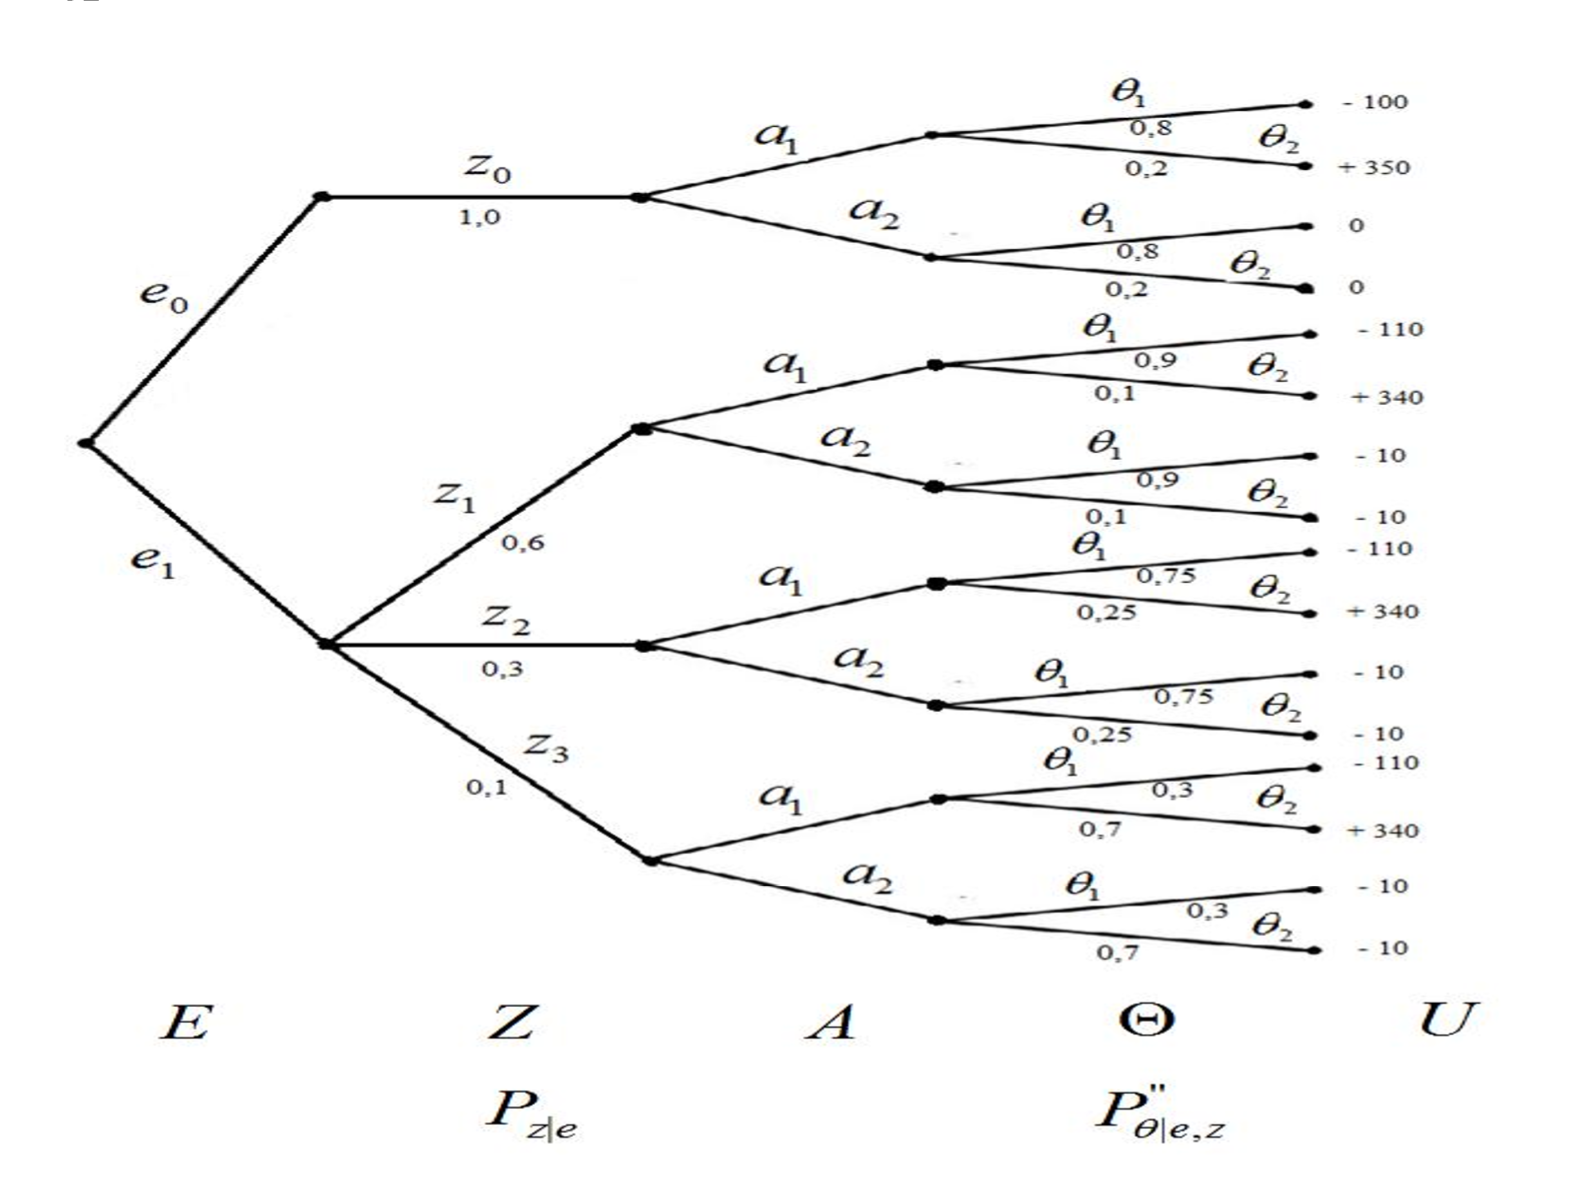
\includegraphics[width=\linewidth]{tree}
    \caption{Дерево решений}
    \label{fig:tree}
\end{figure}

\section*{Выводы}
В ходе лабораторной работы были сформированы навыки принятия управленческих
решений. Для принятия решения использовался метод \enquote{Принятие\\
управленческих решений}.

\end{document}